\documentclass[a4paper, 12pt, french]{article}
\usepackage[utf8]{inputenc}
\usepackage[T1]{fontenc}
\usepackage{babel}

%Images
\usepackage{graphicx} 
\graphicspath{{src/dev/}}

%Code
\usepackage{listings}
\usepackage{color}

\definecolor{dkgreen}{rgb}{0,0.6,0}
\definecolor{gray}{rgb}{0.5,0.5,0.5}
\definecolor{mauve}{rgb}{0.58,0,0.82}

\lstset{frame=tb,
  language=C,
  aboveskip=5mm,
  belowskip=5mm,
  framesep=3mm,
  showstringspaces=false,
  columns=flexible,
  basicstyle={\small\ttfamily},
  numbers=none,
  numberstyle=\tiny\color{gray},
  keywordstyle=\color{blue},
  commentstyle=\color{dkgreen},
  stringstyle=\color{mauve},
  breaklines=true,
  breakatwhitespace=true,
  tabsize=3
}

%Commandes perso
\newcommand{\hr}{\noindent\rule{13.7cm}{0.4pt}}

%Metas
\title{Reseau}
\author{Elanis - https://github.com/Elanis/LaTeX-cheatsheets}
\date{}

\begin{document}
	\maketitle

	Modèle OSI

	\begin{description}
		\item[Physique]
		\item[Liaison]
		\item[Reseau]
		\item[Transport]
		\item[Application]
	\end{description}

	\section{Introduction}

	« Un réseau est un ensemble d'équipement reliés entre eux et qui échangent des informations »

	\subsection{Echanges sur de longues distances}
	\begin{itemize}
		\item Satellite
		\item Hertzien (TV)
		\item Cable aerien
		\item Antenne Parabolique
		\item Paire torsadée (ADSL, Telephone, etc)
		\item WiMax, Telephonique (2G, 3G, 4G), etc
		\item ...
	\end{itemize}

	\subsection{Echanges sur de courtes/moyennes distances}
	\begin{itemize}
		\item CPL (Courant porteur de ligne): Passage du signal par le reseau éléctrique
		\item NFC (Sans contact): Telephones, Cartes bancaires, Badges, etc
		\item Radio: Bluetooth, WiFi, etc
		\item Femtocell: mini-relai telephonique
		\item Ethernet (de 10 Mbps à 10 Gbps)
		\item ...
	\end{itemize}
	
	\subsection{Internet Mobile}  
	\begin{description}
		\item[2G] GSM/GPRS/EDGE - 384Kbps $\downarrow$ - 188.4Kbps $\uparrow$ - 900-1800 Mhz
		\item[3G] UMTS/3G+ (HSPA+) - 14.4Mbps $\downarrow$ - 5.7Mbps $\uparrow$ - 1900-2100 Mhz
		\item[4G] 4G (LTE) - 100Mbps $\downarrow$ - 50Mbps $\uparrow$ - 800 - 1800 - 2600 Mhz
	\end{description}

	\subsection{Internet Fixe}  
	\begin{description}
		\item[ADSL] 13.7Mbps $\downarrow$
		\item[ADSL 2] 25Mbps $\downarrow$
		\item[VDSL 2] 120Mbps $\downarrow$
		\item[Fibre optique] 200Mbps $\downarrow$
		\item[Internet par satellite] 20Mbps $\downarrow$ - \emph{Note:} Utilisée principalement dans les zones non reliables par les solutions précédentes.
	\end{description}

	\subsection{Le Cloud}

	Le but du cloud esst de "dématerialiser" les systèmes informatiques en les envoyant sur le Web. Il en résulte des problèmes sur le reseau avec tout ce nouveau traffic qui auparavant était local aux reseaux d'entreprise le plus souvent. Il exite néanmoins des solutions:

	\subsubsection{Le Edge Computing}

	L'edge computing est une méthode d'optimisation employée dans le cloud computing qui consiste à traiter les données à la périphérie du réseau, près de la source des données. Il est ainsi possible de minimiser les besoins en bande passante entre les capteurs et les centres de traitement des données en entreprenant les analyses au plus près des sources de données.

	\subsubsection{Le Fog Computing}

	Le fog computing consiste à exploiter des applications et des infrastructures de traitement et de stockage de proximité, servant d'intermédiaire entre des objets connectés et une architecture cloud classique.

	\subsection{Niveaux de service}

	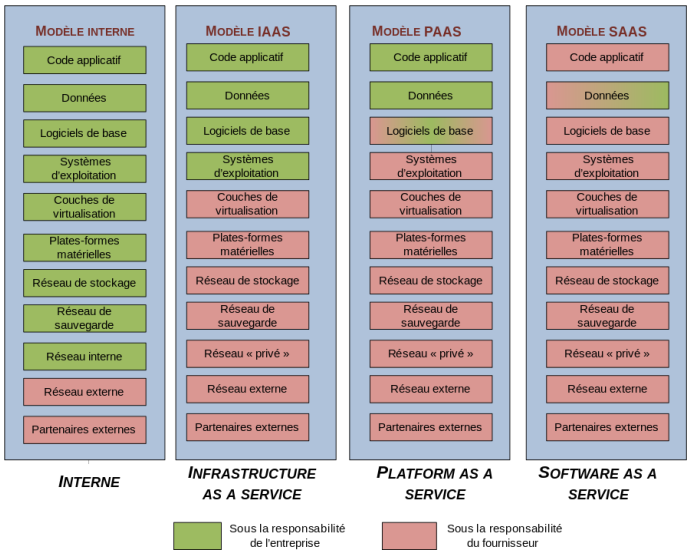
\includegraphics[width=13.8cm]{reseau_niveaux_de_service}
\end{document}